\documentclass[titlepage]{report}
\usepackage[italian]{babel}
\usepackage[babel]{csquotes}
\usepackage[a4paper,left=2cm,bottom=2cm,right=2cm,top=2.5cm]{geometry}
\usepackage[style=numeric-comp,useprefix,hyperref,backend=bibtex,natbib,sorting=none]{biblatex}
\usepackage{subcaption}
\usepackage{url}
\usepackage{graphicx} 			% pacchetto per inserire immagini
\usepackage{sidecap}			% pacchetto delle didascalie laterali
\usepackage{setspace}			% pacchetto per modificare interlinea
\usepackage{textcomp} 			% pacchetto per simboli unicode
\usepackage{float}
\usepackage{hyperref}
\usepackage{fancyhdr}
\usepackage[nowrite,infront,standard,swapnames]{frontespizio}

\begin{document}
	
\hypersetup{
	linkbordercolor={1 1 1},
}

\begin{frontespizio}
	\Universita {Brescia}
	\Logo [3cm]{Logo_unibs.pdf}
	\Dipartimento {Ingengeria dell'Informazione}
	\Corso [Laurea magistrale]{Ingegneria Elettronica}
	\Annoaccademico {2020--2021}
	\Titoletto{Progetto di Sistemi Elettronici Analogici}
	\Titolo {Circuito per la generazione del tono \\ (sinusoidale a frequenza variabile) per Theremin}
	\Sottotitolo{Progetto n°17}
	\NCandidati{Autori}
	\Candidato [706005]{Luca Brescia}
	\Candidato [89521]{Simone Pezzottini}
\end{frontespizio}
	
\tableofcontents

\chapter*{Obiettivo}
	\label{ch:Scope}
	\addcontentsline{toc}{chapter}{Obiettivo}
	\large Realizzazione di un tono a frequenza variabile nello spettro delle frequenze udibili [$20Hz - 20kHz$] utilizzando un VCO e una capacità variabile con il movimento di una mano seguendo lo schema a blocchi mostrato in \textit{Figura \ref{fig:Schema_Assegnazione}}. Il segnale modulato avrà un range di frequenze elevato. Andrà quindi mixato ad una sinusoide a frequenza determinata, per riportare lo spettro del segnale nel range delle frequenze udibili, e opportunamente filtrato per eliminare le componenti indesiderate.
	\\
	\\
	\begin{figure}[h]
		\centering
		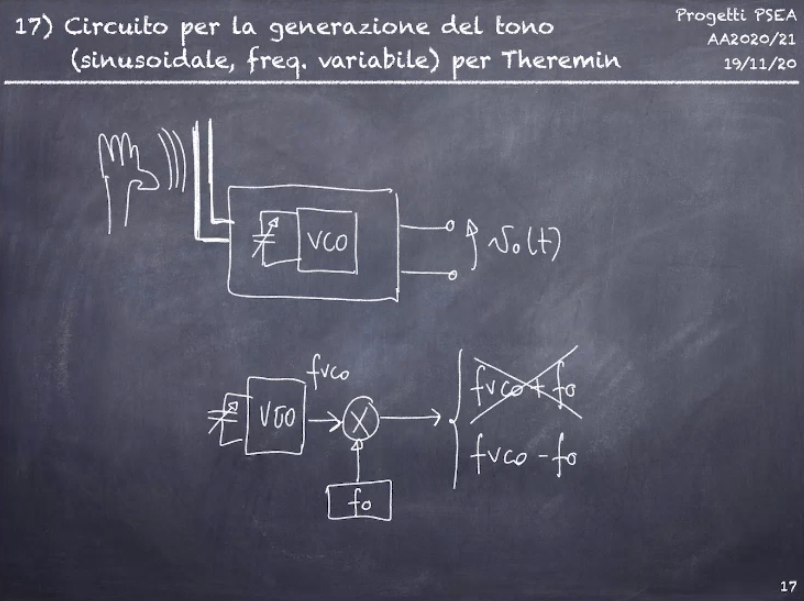
\includegraphics[scale=0.5]{Immagini/Schema_progetto_17.png}
		\caption{Schema generale di funzionamento di un circuito per la realizzazione di un tono.}
		\label{fig:Schema_Assegnazione}
	\end{figure}

	 In generale lo schema richieto per la realizzazione del progetto potrebbe essere il eguente:
	 
	\begin{figure}[htbp]
		\centering
		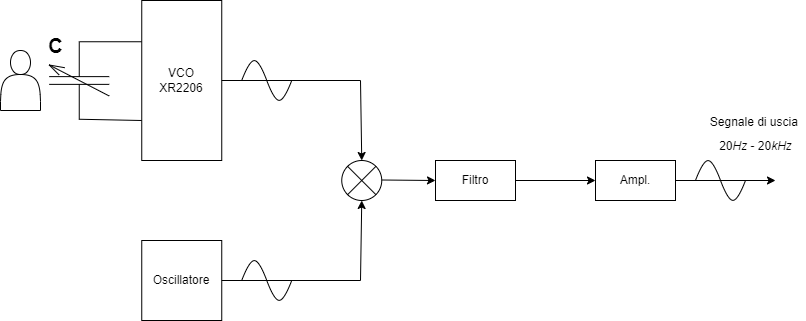
\includegraphics[scale=0.5]{Immagini/Schema Generale PSEA.png}
		\caption{Shema a blocchi generale del progetto}
		\label{fig: schema a blocchi generico}
	\end{figure}


\newpage

	
\chapter{Scelta dei componenti}
	\label{ch:Scelta_componenti}
	I blocchi minimi necessari alla realizzazione di questo progetto sono:
	
	\begin{enumerate}
		\item Oscillatore controllato in tensione $(VCO)$;
		\item Moltiplicatore analogico;
		\item Oscillatore a frequenza fissata;
		\item Filtro passa basso.
	\end{enumerate}
	
	La scelta dei componenti è stata fatta considerando le caratteristiche del segnale da generare. In particolare, volendo realizzare uno shift in frequenza, vi è la necessità di lavorare con integrati con una banda passante adeguata.
	Avendo a disposizione una serie limitata di componenti si è deciso di utilizzare i seguenti componenti:
	
	\begin{enumerate}
		\item l'oscillatore monolitico XR2206 come VCO;
		\item Il moltiplicatore analogico AD633 per lo shift frequenziale;
		\item L'amplificatore operazionale $LF356N$ per la realizzazione dell oscillatore a ponte di Wien per la generazione di una sinusoide di riferimento;
		\item L'amplificatore $LF356P$ per la realizzazione di filtri del segnale.
	\end{enumerate}
	
	
\section{Amplificatori operazionali LF353, LF356 e uA741}
	La scelta di questi due componenti tra quelli disponibili è stata fatta principalmente per le bande.
	\\ Sono necessari componenti a banda elevata poiché dobbiamo lavorare con frequenze dell'ordine delle centinaia di kHz.
	
	 Infatti le bande in gioco sono di circa 3MHz per LF353P mentre 5MHz per LF356N. Ad esempio, il ua741 ha una GBP di 1 MHz tipico.
	
	I due operazionali sono stati scelti per:
	\begin{enumerate}
		\item oscillatore armonica fondamentale
		\item filtro del 4o ordine 
	\end{enumerate}
	
	\noindent I due componenti sono stati scelti in vista dell'oscillatore in quanto le frequenze teoriche sono elevate.	
	
	\noindent Importante osservare che l'LF353P ha al suo interno due amplificatori operazionali per cui è stato scelto per la realizzazione del filtro del 4o ordine.

	\noindent I motivi per cui le frequenze in gioco risultino essere elevate sono indicate nel capitolo \ref{ch:Risultati}.
	
	%Visti i risultati ottenuti a frequenza 250kHz la banda passante potrebbe essere anche inferiore 
	
	%inserire considerazioni su ua741 che abbiamo utilizzato come amplificatore finale (probabilemnte non invertente di guadagno 2 o 3)
	
\section{Oscillatore monolitico XR2206}
	\label{sec:XR2206}
	%pinouut diagram
	
	Si è scelto di utilizzare $XR2206$ perchè permette la generazioni di diverse forme d'onda sinusoidali, onde quadre, rampe, onde triangolari ed impunsi gaarntendo un'alta precisione, stabilità e distorsione. L'ampiezza e la frequenza dei segnali in uscita è direttamente modulabile dall'integrato, gestendo opportunamente gli ingressi. La gamma di frequenze generabili va dai 0.01 $HZ$ a 1 $MHz$, quindi perfetto per le specifiche richieste dal progetto. 
	In \textit{Figura \ref{fig:sch_xr2206}} è mostrato lo schema a blocchi del componente.
	
	\begin{figure}[h]
		\centering
		\subfloat[][\emph{Schema dei collegamenti interni}]
		{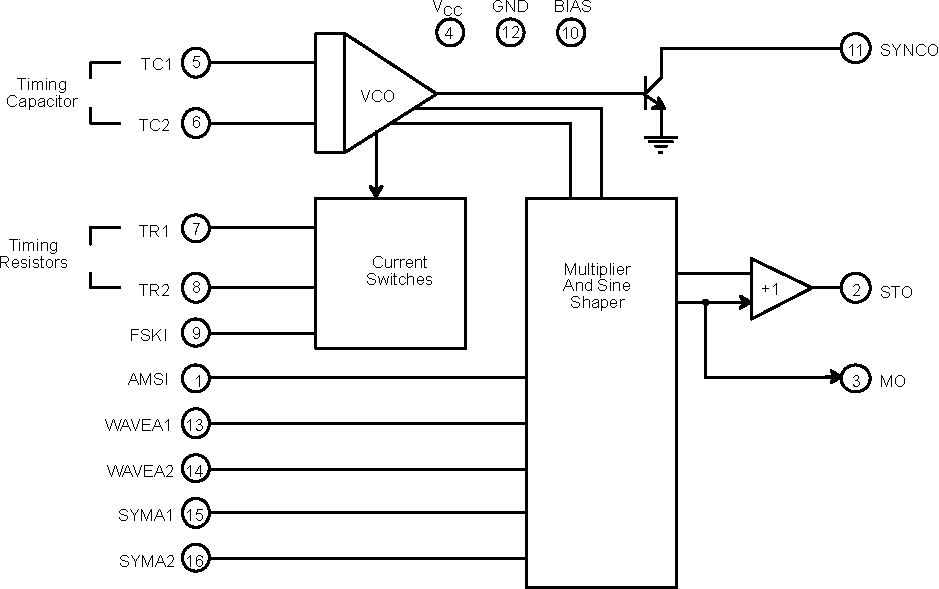
\includegraphics[width=.40\textwidth]{Immagini/schema_blocchi_xr2206.pdf}} \qquad
		\subfloat[][\emph{Descrizione in dettaglio dei pin}]
		{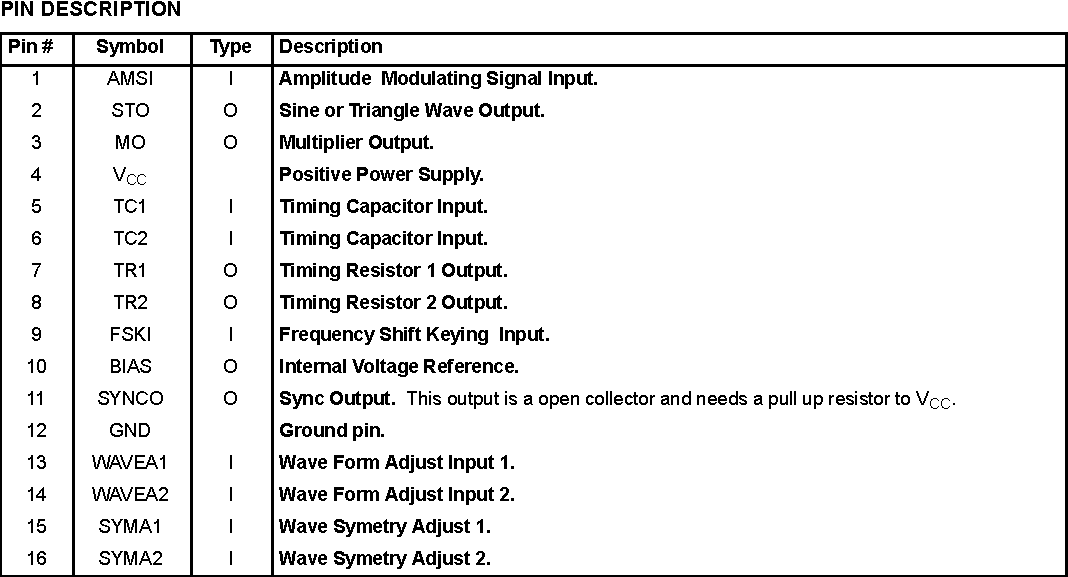
\includegraphics[width=.5\textwidth]{Immagini/schema_blocchi_pinout_xr2206.pdf}} \\
		\caption{Schema a blocchi dell'oscillatore monolitico XR2206}
		\label{fig:sch_xr2206}
	\end{figure}

	La frequenza di oscillazione può essere determinata agendo sulla capacità o sulla resistenza equivlente collegate ai pin opportuni del componente, come riportato nel capitolo \ref{ch:scelte}.
	
	
\section{Moltiplicatore analogico AD633}
	\label{sec:AD633}
	La scelta del moltiplicatore analogico o mixer è stata obbigata in quanto non erano present altri componenti del genera a disposizione.
	Tuttavia garantisce delle buone specifiche permettono di restare nelle specifiche di progetto.
	Infatti possiede elevate impedenze d'ingresso sia sugli ingressi differenziali $X$ e $Y$, che sull'ingersso sommatore $Z$. Una bassa impedenza d'uscita che permette quindi di disaccoppiare la perte a monte del crcuito con quella che si trova a valle. Lavora con una larghezza di banda pari ad 1 $MHz$ e uno slew rate pari a 20 $V/\mu S$. 
	Si può notare , come mostrano in figura \ref{fig:sch_ad633}, che il componete inizia a tagliare ad una frequenza inferiore ripetto alla banda passante teorica indicata; in quanto il taglio inizia intorno ai 500 $kHz$.
	Tuttavia, dal punto di vista teorico, questo non impone una limitazione ai fini del progetto.

	\begin{figure}[h]
		\centering
		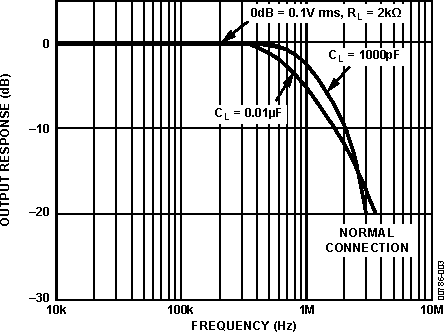
\includegraphics[scale=1]{Immagini/ad633_bp.pdf}
		\caption{Banda passante del moltiplicatore analogico AD633}
		\label{fig:sch_ad633}
	\end{figure}

	\noindent La figura \ref{fig: AD633 schema a blocchi} mostra sai il pinout che lo schema  blocchi interno dell'$AD6333$. Il segnale in uscita dal mixer si calcola con la seguente formula:
	\begin{equation}
		\label{eq: funzione trasferimeto AD633}
		W = \frac{(X1 - X2)(Y1 - Y2)}{10 [V]}  + Z 
	\end{equation}
	Come si può notare dalla formula in segnale viene attenuato di un fattore 10 $V$, quindi sarà necessaria una compensazione del segnale negli stadi successivi. 

	\noindent Analizzando il caso che gli ingressi X2, Y2 e Z collegti a massa, ovvero che diano contributo nullo. L'equazione \ref*{eq: funzione trasferimeto AD633} diventa:
	\begin{equation}
		\label{eq: prodotto sinusoidi AD633}
		W = \frac{X1 * Y1}{10 [V]}
	\end{equation}
	Ora si consideri che i due ingressi siano sinusoidali:
	\begin{equation}
		\label{eq: X1 sinusoidale}
		X1 = A\sin (\omega _1t + \varphi _1)
	\end{equation}
	\begin{equation}
		\label{eq: XY sinusoidale}
		Y1 = B\sin (\omega _2t + \varphi _2)
	\end{equation}
	\begin{equation}
		\label{eq:prodotto sinusoidi con fase}
		W = \frac{AB}{2}[\cos ((\omega _1 - \omega _2)t + (\varphi _1 - \varphi _2)) - \cos ((\omega _1 +\omega _2)t + (\varphi _1 + \varphi _2))]\frac{1}{10[V]}
	\end{equation}
	Aggiungendo l'ipotesi che le due sinusoidi abbiano fase nulla la formula \ref*{eq:prodotto sinusoidi con fase} diventa:
	\begin{equation}
		\label{eq:prodotto sinusoidi}
		W = \frac{AB}{2}[\cos ((\omega _1 - \omega _2)t) - \cos ((\omega _1 +\omega _2)t)]\frac{1}{10[V]} 
	\end{equation}
	Si nota quindi che all'uscita del mixer si avrà un segnale dato dalla combinazione delle due sinusoidi in ingresso, le cui componenti spettrali saranno date una dalla somma delle componenti spettrali delle sinusoidi in ingresso e l'altra dalla loro differenza.
	Quindi inserendo un opportuno filtro passa basso si va a selezionare sollo la componente spettrale d'interesse, ovvero quella compresa tra 20 $Hz$ e 20 $kHz$.

	\begin{figure}[h]
		\centering
		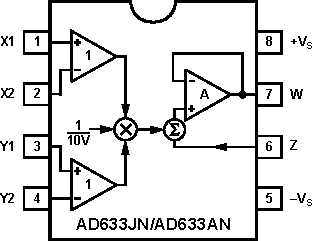
\includegraphics{Immagini/ad633_pinout.pdf}
		\caption{PinOut e schema a blocchi dell'AD633}
		\label{fig: AD633 schema a blocchi}
	\end{figure}

\

\chapter{Scelte progettuali}
	\label{ch:scelte}
	
	Nella realizzazione di questo progetto si deve prestare particolare attenzione allo spettro del segnale di uscita. Nello specifico, si deve valutare il THD della sinusoide di uscita per osservare quanto armoniche indesiderate dovute a disturbi intrinsechi del sistema influiscano sulle performance del dispositivo.
	Per ridurre l'effetto di armoniche a frequenza esterna alla banda udibile si è scelto di introdurre cascate di filtri passa alto e passa basso in modo da cercare un filtro passa-banda accettabile per l'esperienza. Di seguito è riportato lo schema a blocchi del sistema:

	\begin{figure}[h]
		\centering
		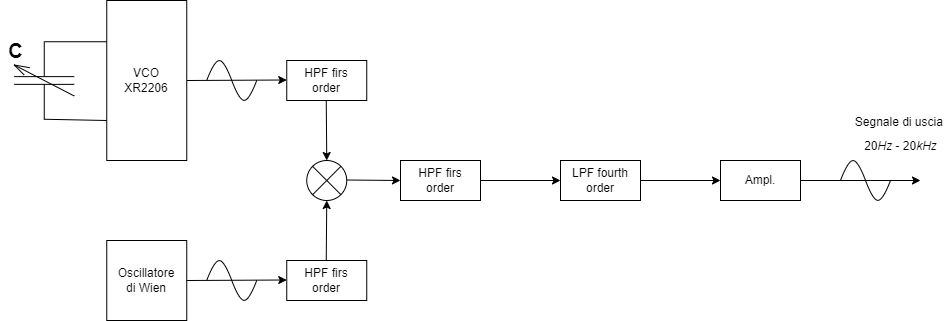
\includegraphics[scale=0.5]{Immagini/Schema a blocchi PSEA.png}
		\caption{Schema a blocchi del sistema realizzato>}
		\label{<fig: Schema a blocchi finale>}
	\end{figure}
\space
	\noindent Nelle sezioni successive vengono analizzati singolarmente le scelte effettuate per ogni singolo blocco del sistema.
	 
\section{VCO}

	Il VCO, \textit{Voltage Controlled Oscillator}, è generatore di segnali che modifica la frequenza di oscillazione del segnale generato in funzione della tensione applicata al suo ingresso.
	
	\noindent La frequenza di oscillazione $f_0$ viene controllata da una capacità esterna C, detta capacità di $timing$ collegata tra i \textit{pin5} e $pin6$ e dalla resistenza R posta in ingresso ai $pin7$ e $pin8$. La frequenza si calcola come:
	
	\begin{equation}
		\label{eq:freq_operation}
		f_0 = \frac{1}{RC} 
	\end{equation}

	\noindent Regolando il valore di \textit{R}, dato dalla somma di $R_1 + 1k\Omega$, e di \textit{C}, si imposta a piacere la frequenza di oscillazione.
	La \textit{Figura \ref{fig:sch_xr2206_}} mostra il circuito utilizzato. Nel progetto si è scelto di utilizzare una resistenza \textit{R} fissa in quanto si ha una capacità variabile per la regolazione della frequenza.

	\begin{figure}[h]
		\centering
		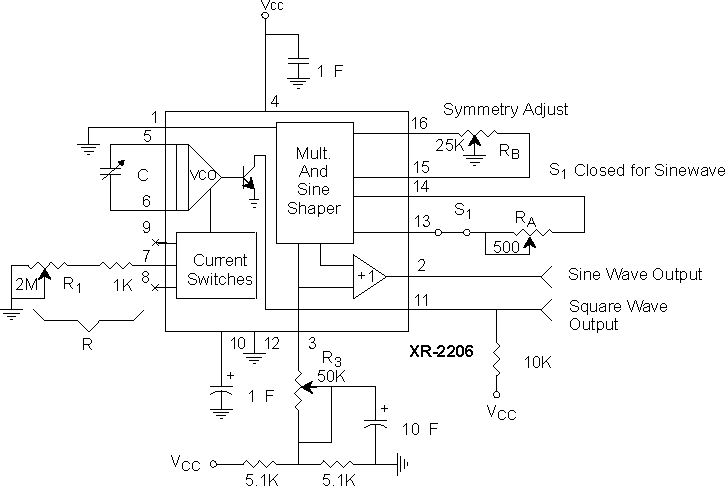
\includegraphics[scale=1]{Immagini/schema_xr2206.pdf}
		\caption{Schema xr2206}
		\label{fig:sch_xr2206_}
	\end{figure}
	\newpage

	\noindent
	Dal datasheet, per garantire una buona stabilità in temperatura, viene consigliato di utilizzare valori di R compresi tra $4k\Omega < R < 200k\Omega$ e valori di C compresi tra $1\mu F < C < 100\mu F$.
	

	% TODO: scrivere i valori corretti
	Dato che la capacità non risulta controllabile, in quanto variabile e data dalla dalla mano dell'utente e dall'antenna realizzata non è controllabile.
	Quindi si è scelta una R di $100k\Omega$ (da verificare). Per la C i risultati sono riportati nel \textit{Capitolo \ref{ch:Risultati}}.
	
\section{Oscillatore sinusoidale di Wien}
	\label{sec:osc_wien}
	Per la realizzazione di un segnale sinusoidale a frequenza fissata si è scelto di utilizzare un oscillatore a ponte di Wien auto-avviante, il cui schema è riportato in \textit{Figura \ref{fig:sch_osc_wien}}
	
	\begin{figure}[h]
		\centering
		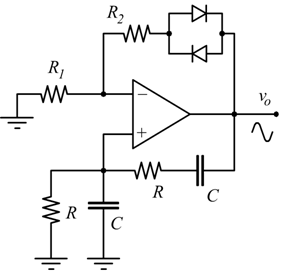
\includegraphics[scale=0.7]{Immagini/sch_osc_wien.png}
		\caption{Schema generale di un oscillatore a ponte di Wien auto-avviante.}
		\label{fig:sch_osc_wien}
	\end{figure}
	
	\noindent Analizzando la $f.d.t$ del circuito si osserva che il prodotto $A\cdot B$ deve essere 1, quindi un numero reale.
	Il blocco di forward A è rappresentato dal guadagno del circuito ovvero: 
	\begin{equation}
		\label{eq:LF356_Gain}
		A = 1 + \frac{R_2}{R_1}
	\end{equation}
	Mentre, in presenza di $R$ e $C$ di valore unico, il blocco di feedback B è rappresentato dall'equazione:
	\\
	\begin{equation}
		\label{eq:LF356_Feedback}
		B = \frac{1}{3 + j\omega C R - j\frac{1}{\omega C R}}
	\end{equation}
	\\
	Per l'innesco delle oscillazioni è necessario che il guadagno ad anello aperto sia inizialmente $A\cdot B>1$ ed $A>3$ per poi assestarsi a $A\cdot B=1$ ed $A=3$. La tecnica più semplice consiste nel disporre due diodi in antiparallelo lungo l'anello di retroazione dell'OpAmp.
	
	\noindent Quando \textit{$V_{O}$} è bassa i diodi presentano un'alta resistenza differenziale mentre all'aumentare di \textit{$V_{O}$} essa diminuisce. 
	\\ Per rispettare le condizioni di lavoro imposte, il guadagno A può essere posto, circa, all'85\% del suo valore nominale (A=2,5 — 2,55) così si fa in modo modo che $A>3$ all'avvio che poi si riduce ad A=3 a regime.

	\begin{figure}[h]
		\centering
		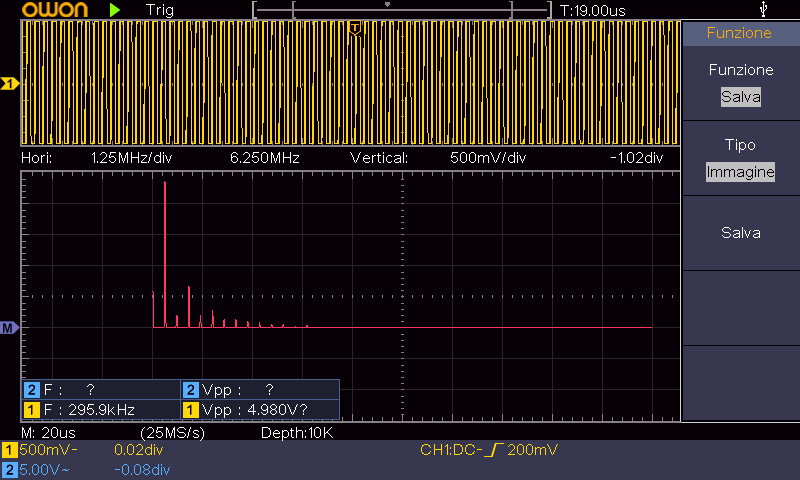
\includegraphics[scale=0.9]{Immagini/009_OscillatoreWienFFT.png}
		\caption{FFT della sinusoide a 295kHz in uscita dall'oscillatore acquisita tramite oscilloscopio}
		\label{fig:FFT295k}
	\end{figure}
	
	Dalla \textit{Figura \ref{fig:FFT295k}} si può notare la presenza di sole due armoniche: quella voluta a 295kHz e una componente in continua. \\
	La componente in continua è sicuramente dovuta alla strumentazione utilizzata poiché anche introducendo un elemento capacitivo per disaccoppiare, la componente è sempre rimasta presente.
	Per la valutazione della distorsione della sinusoide ottenuta si utilizza il calcolo del THD riportato nell'equazione:
	
	\begin{equation}
		\label{eq:thd}
		THD (\%) = 100 \cdot \frac{\sqrt{\sum_{2}^{\infty} V_{n}^2}}{V_1}
	\end{equation}

	Tutti i valori di tensione devono essere in RMS: 
	
	\begin{equation}
		\label{eq:Vrms}
		V_{RMS} = \frac{V}{\sqrt{2}}
	\end{equation}

	%% OSS: L'oscillatore di Wien è sensibile alle temperature, l'ampiezza dell uscita varia in funzione della temperatura (detto a lezione)

	% Se la distorsione non è armonica cosa succede? Ottendo piu righe spettrali che mi generano disturbi nel segnale
	
	% Cosa succede se la distorsione è sull'amplificatore, piuttosto che sull'oscillatore piuttosto che sull'XR? Bisogna che i componenti siano a bassa distorsione armonica.
	
	% Se il segnale in uscita all'oscillatore di wien fosse triangolare, cosa accade dopo il motiplicatore? Prossima lezione si vedrà cosa accade se il segnale è un onda quadra.
		
\newpage
\section{Moltiplicatore analogico}
	Alla moltiplicazione di due segnali nei tempi corrisponde la convoluzione degli stessi in frequenza. Questo porta ad ottenere due sinusoidi centrate a frequenza $\omega_1 + \omega_2$ e $\omega_1 - \omega_2$.
	
	In \textit{Figura \ref{fig:FFTmixer}} viene mostrato il risultato ottenuto moltiplicando la sinusoide ottenuta precedentemente \textit{Sezione \ref{sec:osc_wien}} con l'oscillatore di Wien e una sinusoide generata dal generatore di funzione ad una frequenza di 20 kHz.
	
	\begin{figure}[h]
		\centering
		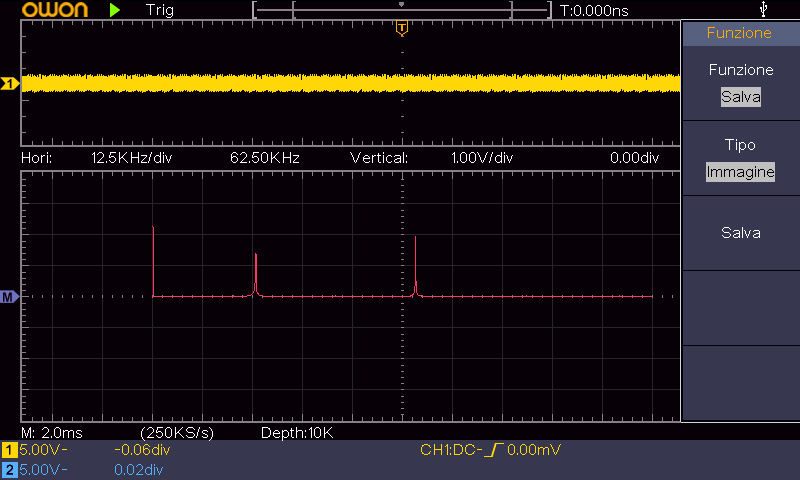
\includegraphics[scale=0.9]{Immagini/uscita_ad633_con_fcngen_20k_e_osc_45k.png}
		\caption{FFT del segnale in uscita dall'AD633}
		\label{fig:FFTmixer}
	\end{figure}
	
	 Essendo i due segnali in gioco di 20kHz e 45kHz, dalla  \textit{Figura \ref{fig:FFTmixer}}	si può notare come vengano generate due sinusoidi aventi armoniche fondamentali a $(45-20)kHz$ e $(45+20)kHz$ escludendo la componente armonica a frequenza nulla che è generata dalla strumentazione come spiegato in precedenza.
	 \\
	 Inoltre, le ampiezze rilevate risultano in linea con i risultati teorici in quanto l'ampiezza di picco dei due segnali in gioco è di $12V$ e $2.5V$ rispettivamente che vengono moltiplicate tra loro e divise di un fattore $10$ come specificato nel datasheet del componente. Si nota anche come le due ampiezze non siano uguali: questo è un errore dovuto alla non-linearità del componente. Tuttavia, per la nostra applicazione questo errore è irrilevante in quanto ci interessa maggiormente la componente armonica del segnale.
	
\newpage
\section{Filtro LP del quarto ordine}
	Il prodotto di due sinusoidi del mixer porterà in uscita due sinusoidi a frequenze diverse ovvero una sarà $\omega_{wien} + \omega_{VCO}$ e l'altra a $\omega_{wien} - \omega_{VCO}]$. Per rientrare nelle specifiche di progetto, è stato necessario introdurre un filtro passa-basso (LP) tale che permettesse di avere in uscita solo la componente armonica $\omega_{wien} - \omega_{VCO}$.
	\\ 
	Volendo un filtro molto selettivo e visto che il compondente $LF353P$ ha al suo interno due amplificatori, si è scelto di utilizzare un filtro attivo di ordine 4. Realizzandolo tramite un filtro di Chebychev con due configurazioni Sallen-Key in casacata. 
	
	\begin{figure}[h]
		\centering
		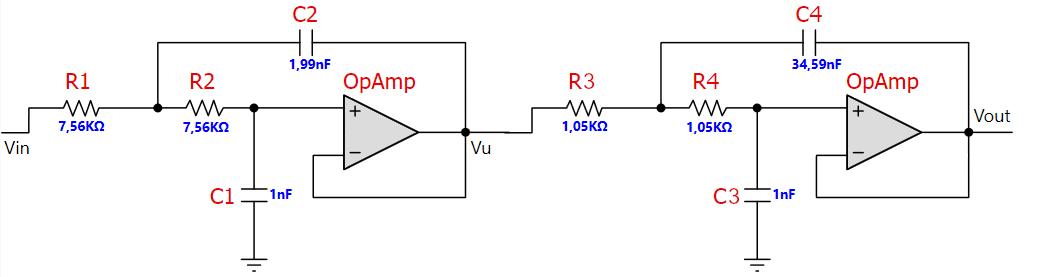
\includegraphics[scale=0.9]{Immagini/sch_lp4.png}
		\caption{Filtro attivo di ordine 4.}
		\label{fig:LP4}
	\end{figure}	
	
	Dove la sua risposta in frequenza del modulo del filtro teorico risulta essere quello riportato nella \textit{Figura \ref{fig:BodeLp4}}.
	
	\begin{figure}[h]
		\centering
		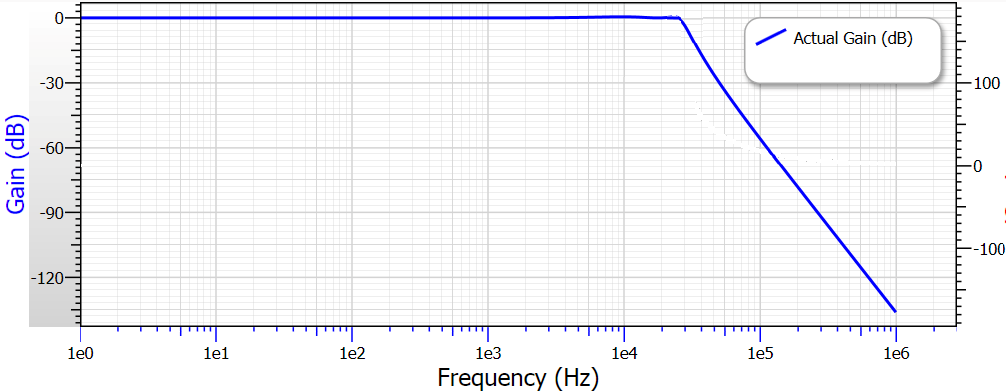
\includegraphics[scale=0.9]{Immagini/bode_teorico_lp4.png}
		\caption{Diagramma di Bode del modulo del filtro.}
		\label{fig:BodeLp4}
	\end{figure}


\chapter{Risultati sperimentali}

\section{XR2206}
	Per la realizzazione dell'armonica a frequenza variabile ci siamo appoggiati al datasheet del componente scegliendo come valori di partenza quelli mostrati in esempio. 
	
	La capacità variabile è stata realizzata con un supporto rigido e della carta di alluminio posta a bandiera. Il tutto è stato collegato come mostrato in figura.
	
	% TODO:inserire foto circuito XR2206 con antenna.
	
	Le prestazioni ottenute con questo tipo di antenna sono le seguenti:
	
	% TODO: Foto distanza misurata della mano (senza mano, dove comicia a variare, variazione massima)
	
	
\section{AD633}
	
	%Verificare il limiti operativi del componente.
	
	Verifichiamo il THD delle sinusoidi in uscita dall'Oscillatore e AD633
	Osserviamo che in entrambi i casi non otteniamo distorsioni. Notiamo una continua di circa 2V che non riconosciamo.
	Aggiungendo un condensatore di filtraggio in uscita al moltiplicatore non otteniamo risultati. Ipotizziamo sia dovuto a qualcosa di intrinseco all'oscilloscopio. 
	Anche perché nella visualizzazione della sinusoide non rileviamo alcun offset. Inoltre ad un certo punto delle misurazioni è sparito.
	Abbiamo osservato che l'ampiezza delle righe della fft è coerente con i segnali in ingresso al sistema. $V_{osc}$=15V $V_{fcngen}$=2.5V quindi considerando il fattore intrinseco di scala dell'AD633 otteniamo delle righe di fft di ampiezza coerente perché sommando le varie componenti si ottiene quei 3.5V circa di ampiezza del segnale.

	\begin{figure}[h]
		\centering
		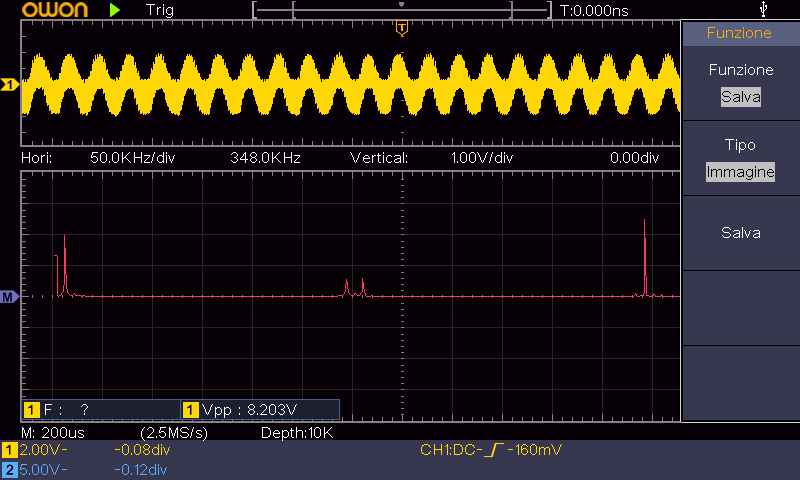
\includegraphics[scale=0.9]{Immagini/AD633_300k.png}
		\caption{FFT in uscita dall'AD633 con fondamentale a 300k}
		\label{fig:FFTAD633}
	\end{figure}

	\label{ch:Risultati}
	
	% TODO: Qui tutta la pappa con le immagini oscilloscopio e breadboard, qualche calcolo anche excel e tanta ma tanta descrizione che non serve a nulla

\newpage
\section{LP4}
	% TODO: Inserire diagramma di bode sperimentale.
	
	% TODO: Inserire un diagramma per punti mettendo in ingresso al filtro un segnale con il generatore di funzioni variando la F di X kHz e visualizzando l'uscita sull'oscilloscopio
	\subsection{Analisi della banda in anello chiuso}
	     \begin{figure}[h]
	     	\centering
	     	\subfloat[][\emph{Didascalia figura }]
	     	{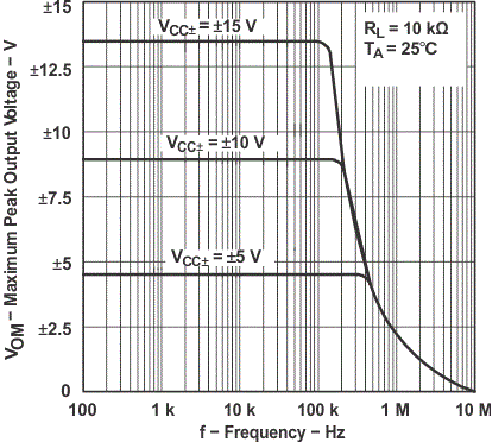
\includegraphics[width=.45\textwidth]{Immagini/lf353p_performance.pdf}} \qquad
	     	\subfloat[][\emph{Didascalia figura}]	     	{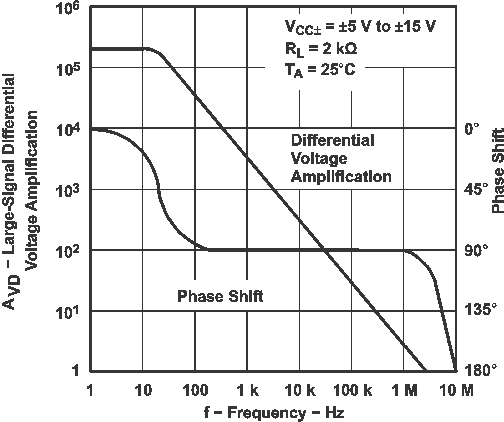
\includegraphics[width=.49\textwidth]{Immagini/bode_lf353p.pdf}} \\
	     	\caption{Diagrammi di bode del componente LF353P in anello aperto}
	     	\label{fig:bode_LF353P}
	     \end{figure}
     	% TODO: Testare il filtro passa alto che porta essere posizionato o in fondo prima o dopo del 741, oppure tra il mixer e il filtro del 4o ordine.
     	
     	%% Conti sul rumore non ce ne servono      
\section{Theremin}
	%Schematico con cad
	
	%Considerazioni sul circuito: scelta della frequenza di oscillazione
	%che è stata cambiata perchè non riuscivamo a farla variare con la mano ecc...
	
	%
\chapter{Conclusioni}
 	\label{ch:Conclusioni}
	Bene questo progetto si conclude qui, \textit{grazie a tutti!}
	
	
\end{document}
